\documentclass[10pt,a4paper]{article}

%%%%%%%%%%%%%%%%%%%%%%%%%%%
% MODIFY:

\newcommand{\authorA}{Ahmad Bin Qasim (03693345)}
\newcommand{\authorB}{Kaan Atukalp (03709123)}
\newcommand{\authorC}{Martin Meinel (03710370)}
\newcommand{\groupNumber}{H} % - YOUR GROUP NUMBER
\newcommand{\exerciseNumber}{2} % - THE NUMBER OF THE EXERCISE
\newcommand{\sourceCodeLink}{https://gitlab.lrz.de/ga53rog/praktikum-ml-crowd}

\newcommand{\workPerAuthor}{
\authorA&Task 1&33\%\\
      &Task 2&33\%\\
      &Task 3&33\%\\
      &Task 4&33\%\\
      &Task 5&33\%\\
      \hline
\authorB&Task 1&33\%\\
      &Task 2&33\%\\
      &Task 3&33\%\\
      &Task 4&33\%\\
      &Task 5&33\%\\
      \hline
\authorC&Task 1&33\%\\
      &Task 2&33\%\\
      &Task 3&33\%\\
      &Task 4&33\%\\
      &Task 5&33\%\\
}

%%%%%%%%%%%%%%%%%%%%%%%%%%%

%%
% imports for the exercise sheets
%

\usepackage[utf8]{inputenc}
\usepackage{amsmath}
\usepackage{amsfonts}
\usepackage{amssymb}

\usepackage[yyyymmdd]{datetime}
\renewcommand{\dateseparator}{--}

\usepackage[left=2cm,right=2cm,top=3cm,bottom=3cm]{geometry}

\usepackage{hyperref}

\usepackage{amsthm}
\newtheorem{lem}{Lemma}
\newtheorem{thm}{Theorem}
\newtheorem{cor}{Corollary}
\newtheorem{rem}{Remark}
\newtheorem{definition}{Definition}
\newtheorem{ter}{Terminology}

\usepackage{graphicx}

\newcommand{\M}{\mathcal{M}}
\newcommand{\N}{\mathcal{N}}
\newcommand{\K}{\mathcal{K}}
\newcommand{\SPDk}{\mathbb{P}^k}
\newcommand{\vol}{\text{vol}}

\newcommand{\Figref}[1]{Figure~\ref{#1}}
\newcommand{\figref}[1]{figure~\ref{#1}}
\newcommand{\Eqnref}[1]{Equation~(\eqref{#1})}
\newcommand{\eqnref}[1]{equation~(\eqref{#1})}

\usepackage{float}
\usepackage{tabularx}
\usepackage{subcaption}
\usepackage{mwe}

\usepackage{fancyhdr}
\pagestyle{fancy}

\usepackage{totcount}
\newtotcounter{taskCounter}
\newtotcounter{pointCounter}
\newenvironment{task}[1]{\noindent\stepcounter{taskCounter}\textbf{Report on task #1}\smallbreak\hrule\smallbreak}{\smallbreak\hrule\bigbreak}


\title{Report for exercise \exerciseNumber~from group~\groupNumber}

\makeatletter
\let\thetitle\@title
\let\theauthor\@author
\let\thedate\@date
\makeatother

\providecommand{\versiondate}{\today}

\lhead{Exercise sheet \exerciseNumber}
\chead{Master Praktikum: Modelling and Simulation of Crowds WS2019/20}
\rhead{TUM}
\lfoot{Report of Group \groupNumber}
\cfoot{\thepage}
\rfoot{Last compiled: \versiondate}
\renewcommand{\headrulewidth}{0.4pt}
\renewcommand{\footrulewidth}{0.4pt}

\newcommand{\frontpage}{
\begin{center}
\textbf{\thetitle}\\~\\
\end{center}
\begin{table}[H]
\begin{tabular}{ll}
Tasks addressed:&\total{taskCounter}\\
Authors:&\authorA\\
&\authorB\\
&\authorC\\
Last compiled:&\versiondate\\
Source code:&\sourceCodeLink
\end{tabular}
\end{table}
\vfill
The work on tasks was divided in the following way:
\begin{table}[H]
\begin{tabularx}{\textwidth}{X|p{2cm}|p{2cm}}
\workPerAuthor
\end{tabularx}
\end{table}
\newpage
}

\begin{document}

\frontpage

\begin{task}{1, Vector fields, orbits, and visualization}
\end{task}
\begin{task}{2, Common bifurcations in nonlinear systems}
     \begin{figure}[H]
        \centering
        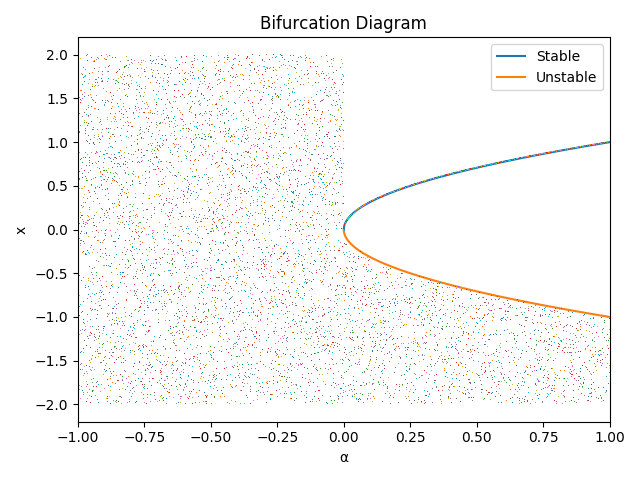
\includegraphics[width=0.7\textwidth]{../plots/task2_1.png}
        \caption{The bifurcation diagram for equation 6 with $\alpha$ in (-1,1)}
        \label{fig:task2_1_bifurcation}
    \end{figure}    
    \begin{figure}[H]
        \centering
        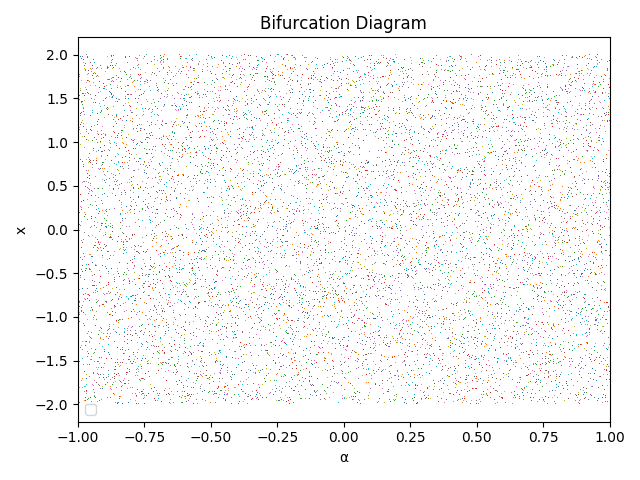
\includegraphics[width=0.7\textwidth]{../plots/task2_2.png}
        \caption{The bifurcation diagram for equation 7 with $\alpha$ in (-1,1)}
        \label{fig:task2_2_bifurcation}
    \end{figure}
	
	We know that, for two dynamical systems to be topologically equivalent, there should exist homeomorphism of the parameter space and a parameter-dependent homeomorphism of the phase space.
	
	\begin{enumerate}
		\item The bifurcation that occurs at $\alpha=0$ is, saddle node bifurcation.
		\item The dynamical systems explained by equation 6 and 7 are not topologically equivalent for $\alpha=1$ because, although they have the same normal form. The dynamical system explained by equation 7 has no steady state for $\alpha=1$, instead the steady state of the dynamical system in question exists at $x0 = \pm \sqrt{\frac{\alpha -2}{2}}$ only for $\alpha > 2$ as shown by figure \ref{fig:task2_3_bifurcation}. According to the definition of topological equivalence mentioned before, for $\alpha=1$ the parameter-dependent homeomorphism of the phase space does not exist.
		\item The dynamical systems explained by equation 6 and 7 are not topologically equivalent for $\alpha=-1$ as well, because at $\alpha=-1$ neither of the dynamical systems have any steady states.
	\end{enumerate}	        
    
    \begin{figure}[H]
        \centering
        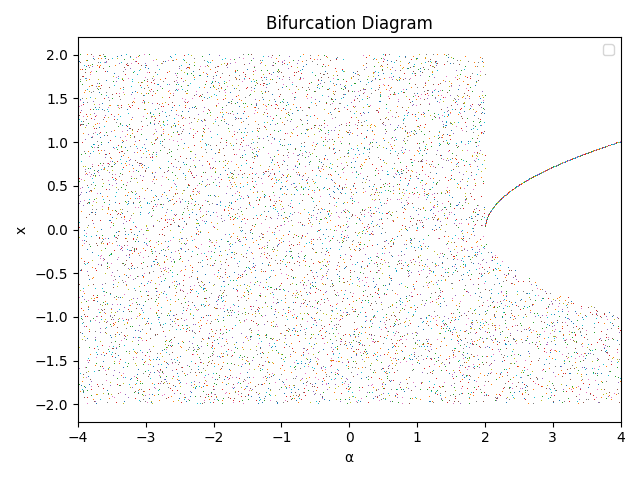
\includegraphics[width=0.7\textwidth]{../plots/task2_3.png}
        \caption{The bifurcation diagram for equation 7 with $\alpha$ in (-4,4)}
        \label{fig:task2_3_bifurcation}
    \end{figure}
\end{task}
\begin{task}{3, Bifurcations in higher dimensions}
\end{task}
\begin{task}{4, Chaotic dynamics}
\end{task}
\begin{task}{5, Bifurcations in crowd dynamics}
\end{task}

\end{document}
